\documentclass[12pt]{article}
\usepackage[utf8]{inputenc}
\usepackage[T1]{fontenc}
\usepackage{amsmath}
\usepackage{amsfonts}
\usepackage{amssymb}
\usepackage[version=4]{mhchem}
\usepackage{stmaryrd}
\usepackage{graphicx}
\usepackage[export]{adjustbox}
\usepackage{caption}
\usepackage{geometry}
\usepackage{hyperref}
\graphicspath{{./figures/}}

\geometry{
    margin=1in,
    textwidth=6.5in,
    textheight=9in
}

\begin{document}
\captionsetup{singlelinecheck=false}
\section*{Problem Set 2}
Due: Wednesday $10 / 1 / 25$ at the start of class\\
Feel free to use any resource to work these problems, including books, websites, and your classmates. However, your problem set submission must be your own work.

\section{Problem 1. Solid-Oxide Fuel Cells}
Solid oxide fuel cells (SOFC) involve a solid ceramic electrolyte. Advantages of SOFCs include fuel flexibility, use of cheaper catalysts, high power densities, and high quality waste heat for cogeneration. Physically, a SOFC conducts $\mathrm{O}^{2-}$ anions through a solid electrolyte, replacing the proton and hydroxide conductors we discussed in class. In order to be conductive for $\mathrm{O}^{2-}$ ions, these cells must be operated at high temperatures.\\
\subsection{}
 Draw a solid oxide fuel cell given a feed of hydrogen and oxygen. Label the reactants and products, write out the half reactions, draw the path of the electrons in an external circuit, and indicate the direction of movement of the $\mathrm{O}^{2-}$ ion in the solid electrolyte.\\
\subsubsection{Solution}
Given it is difficult for me to draw, so \ref{sofc_h2} which does this drawing and I annotate it.
\begin{figure}[h!]
    \centering
    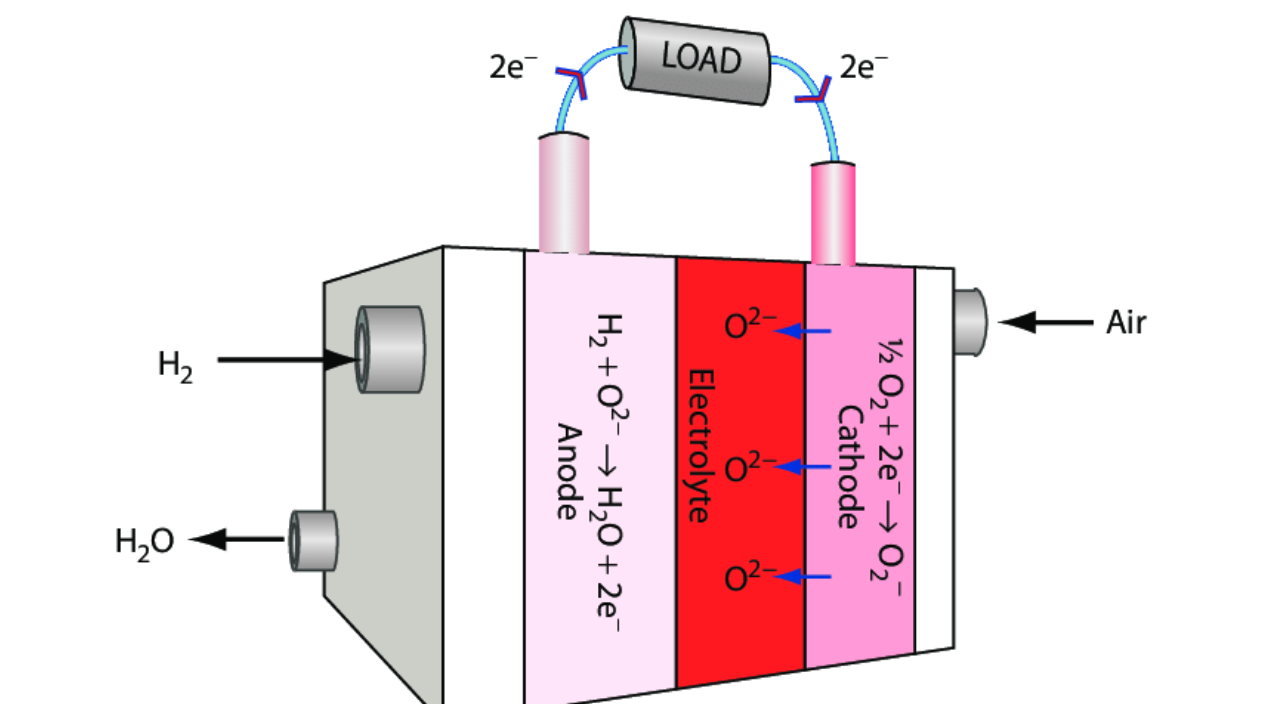
\includegraphics[width=\textwidth]{SOFC_h2.png}
    \caption{So the reactants are hydrogen and oxygen gas, with the product being water. The half reaction at the cathode is $ \mathrm{O}_{2} + 4 \mathrm{e}^{-} \rightarrow 2 \mathrm{O}^{2-}$ and at the anode, we have $2 \mathrm{H}_{2} + 2 \mathrm{O}^{2-} \rightarrow 2 \mathrm{H}_{2} \mathrm{O} + 4 \mathrm{e}^{-}$. The electrons move through the external circuit from the anode to the cathode, while the $\mathrm{O}^{2-}$ ions move through the solid electrolyte from the cathode to the anode.}
\label{sofc_h2}
\end{figure}



\subsection{}
b) Repeat the above for feeds of methane and oxygen to the anode and cathode, respectively (remember that the cell is operating at very high temperatures; what is the electrochemically active feed?).
\subsubsection{Solution}
See \ref{sofc_ch4} for the drawing.
\begin{figure}[h!]
    \centering
    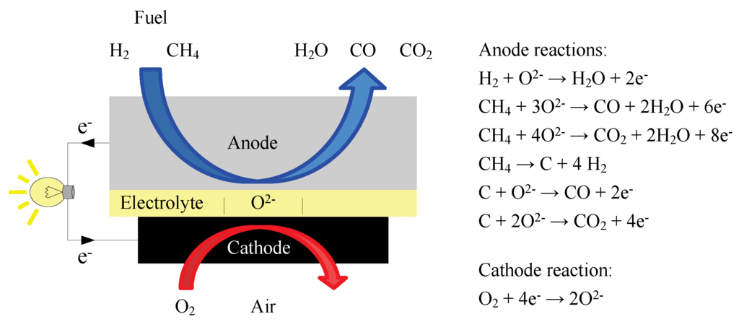
\includegraphics[width=\textwidth]{SOFC_methane.png}
    \caption{At the high temperatures, the methane will decompose as $ \mathrm{CH}_{4} \rightarrow \mathrm{C} + 2 \mathrm{H}_{2}$, and then, as indicated, at the anode we can have the previous hydrogen reaction producing water, but we can also have the conversion of the elemental carbon into $CO_2$. The movement of electrons and $\mathrm{O}^{2-}$ ions is the same as in the previous case.}
\label{sofc_ch4}
\end{figure}

Use your result from (a) for the rest of the problem.\\
\subsection{}
c) Using values for the thermodynamics of each species found in NIST, write out an expression for the open circuit potential of the cell as a function of temperature. Please state all assumptions clearly.\\
\subsubsection{Solution}
We will make the assumption that all quantities of formation are temperature independent, so that we can just use the ones at the standard state.
\begin{center}
\begin{tabular}{|c|c|c|c|}
\hline
 & $H_{2}(g)$ & $O_{2}(g)$ & $H_{2}O(g)$ \\
\hline
$\Delta H_{f}^{\circ}$ (kJ/mol) & 0 & 0 & -241.8 \\
\hline
$S^{\circ}$ (J/mol$\cdot$K) & 130.6 & 205.2 & 188.7 \\
\hline
\multicolumn{4}{|c|}{Reaction: $H_{2}(g) + \frac{1}{2} O_{2}(g) \rightarrow H_{2}O(g)$} \\
\hline
\end{tabular}\\
\end{center}
% 1.2530445146914 - 0.000230605793646681⋅T
The computation I did in my notebook says that my OCV expression is:

$$
E_{cell} = 1.253 - 2.306 \times 10^{-4} \cdot T
$$
\subsection{}
d) In practice, there is significant ionic resistance in the electrolyte, particularly at lower temperatures. Given the following expression for electrolyte conductivity, write out a complete expression for the cell voltage as a function of temperature, accounting for ionic resistive losses due to $\mathrm{O}^{2-}$ conduction, but ignoring all other loss mechanisms.

$$
\sigma(S / \mathrm{cm})=A \cdot \exp \left[\frac{E}{R}\left(\frac{1}{T_{0}}-\frac{1}{T}\right)\right]
$$

For $\mathrm{Y}_{2} \mathrm{O}_{3}$-doped $\mathrm{ZrO}_{2}\left(8 \% \mathrm{Y}_{2} \mathrm{O}_{3}\right), A=0.14 S / \mathrm{cm}$ and $E=75 \mathrm{~kJ} / \mathrm{mol}$ at $1000^{\circ} \mathrm{C}$ (Arachi et al. Solid State Ionics. 121 (1999)). While conditions vary depending on the material and the exact desired optimization, for our purposes assume the solid electrolyte is 150 microns thick. Assume the current is $500 \mathrm{~mA} / \mathrm{cm}^{2}$.\\
\subsubsection{Solution}
So the total potential will consist of the difference petering the Nernst potential and the resistive losses, so we have:
\begin{align}
    V_{cell} &= E_{cell} - iR = E_{cell} - i \frac{L}{\sigma A} = E_{cell} - i \frac{L}{A} \frac{1}{\cdot \exp \left[\frac{E}{R}\left(\frac{1}{T_{0}}-\frac{1}{T}\right)\right]} \\
\end{align}
And we have $L = 150 \times 10^{-4} cm, i = 500 \frac{mA}{cm^{2}}\times \frac{1 A}{1000 mA}, A = 0.14 \frac{S}{cm}, E = 75000 \frac{J}{mol}, R = 8.314 \frac{J}{K \cdot mol}, T_0 = 1273 K$. From my notebook, I get an expression for
\begin{equation}
    V_{cell} = -2.306 \times 10^{-4} \cdot T - 4.481 \times 10^{-5} \cdot \exp\left(\frac{9020.93}{T}\right) + 1.253
\end{equation}
% -0.000230605793646681*T - 4.48093680057448e-5*exp(9020.92855424585/T) + 1.2530445146914
\subsection{}
e) Plot of cell voltage as a function of temperature. What temperature does the maximum potential occur at and what is that potential? How does this optimal temperature change for: (i) $1 \mathrm{~A} / \mathrm{cm} 2$, (ii) $A=0.014 \mathrm{~S} / \mathrm{cm}$, (iii) $A=1.4 \mathrm{~S} / \mathrm{cm}$
\subsubsection{Solution}
See the plots for the values.

\section{Problem 2. Corrosion Currents}
Under some conditions, corrosion can refer to a spontaneous chemical reaction that results from a neutral combination of Faradaic reactions (redox couple) at the same electrode. Since no electron must pass through the external circuit, corrosion can occur under open circuit conditions. For example, in a lead-acid battery, the corrosion reaction

$$
\mathrm{Pb}^{2+}+\mathrm{SO}_{4}^{2-} \rightarrow \mathrm{PbSO}_{4}(\mathrm{~s})
$$

can occur at both electrodes. At the anode, the half reaction


\begin{equation*}
\mathrm{Pb}(s)+\mathrm{SO}_{4}^{2-} \rightarrow \mathrm{PbSO}_{4}(s)+2 e^{-}, \phi_{1}^{\Theta}=-0.356 \mathrm{~V} \tag{1}
\end{equation*}


couples to lead electrodeposition,


\begin{equation*}
P b^{2+}+2 e^{-} \rightarrow P b(s), \phi_{2}^{\Theta}=-0.126 V \tag{2}
\end{equation*}


and at the cathode, the half reaction


\begin{equation*}
\mathrm{PbO}_{2}(s)+\mathrm{SO}_{4}^{2-}+4 \mathrm{H}^{+}+2 e^{-} \rightarrow \mathrm{PbSO}_{4}(s)+2 \mathrm{H}_{2} \mathrm{O}, \phi_{3}^{\Theta}=1.685 \mathrm{~V} \tag{3}
\end{equation*}


couples to lead oxide electrodeposition,


\begin{equation*}
\mathrm{Pb}^{2+}+2 \mathrm{H}_{2} \mathrm{O} \rightarrow \mathrm{PbO}_{2}(\mathrm{~s})+4 \mathrm{H}^{+}+2 e^{-}, \phi_{4}^{\Theta}=1.455 \mathrm{~V} \tag{4}
\end{equation*}


With these coupled reactions, there is no net passage of charge at each electrode despite the fact that charge transfer reactions are occurring at the electrode surface.\\
\subsection{}
a) For each reaction ( $i=1,2,3,4$ ), relate the equilibrium electrode potential $\phi_{i}$ vs. the standard hydrogen electrode (SHE) to $p H, p\left[\mathrm{SO}_{4}^{2-}\right]$, and $p\left[\mathrm{~Pb}^{2+}\right]$, assuming that the other reactants have unit activities. ( $p[$ ion $]=-\log _{10}[$ ion $]$ )\\
\subsubsection{Solution}
My notebook gives (all in units of V):
% For phi_ref = -0.356 V:
% 0.029563250007874⋅pSO42m - 0.356
% For phi_ref = -0.126 V:
% 0.029563250007874⋅pPb2p - 0.126
% For phi_ref = 1.685 V:
% 0.118253000031496⋅pHp + 0.029563250007874⋅pSO42m + 1.685
% For phi_ref = 1.455 V:
% -0.118253000031496⋅pHp + 0.029563250007874⋅pPb2p + 1.455
\begin{align}
    \phi_1 &= 2.956 \times 10^{-2} \cdot p\left[\mathrm{SO}_{4}^{2-}\right] - 0.356 \\
    \phi_2 &= 2.956 \times 10^{-2} \cdot p\left[\mathrm{~Pb}^{2+}\right] - 0.126 \\
    \phi_3 &= 1.183 \times 10^{-1} \cdot pH + 2.956 \times 10^{-2} \cdot p\left[\mathrm{SO}_{4}^{2-}\right] + 1.685 \\
    \phi_4 &= -1.183 \times 10^{-1} \cdot pH + 2.956 \times 10^{-2} \cdot p\left[\mathrm{~Pb}^{2+}\right] + 1.455
\end{align}
\subsection{}
b) Assume that the anode potential is $\phi_{a}=\frac{\phi_{1}+\phi_{2}}{2}$ and the cathode potential is $\phi_{c}=\frac{\phi_{3}+\phi_{4}}{2}$ (we will derive in the kinetics section!) What is the open circuit potential as a function of $p H, p\left[\mathrm{SO}_{4}^{2-}\right]$, and $p\left[\mathrm{~Pb}^{2+}\right]$.\\
\subsubsection{Solution}
my notebook gives (in V):
% 1.811
\begin{equation}
    E_{cell} = \phi_c - \phi_a = 1.811
\end{equation}
So the open circuit potential is independent of $pH, p\left[\mathrm{SO}_{4}^{2-}\right]$, and $p\left[\mathrm{~Pb}^{2+}\right]$.
\subsection{}
c) If the sulfuric acid concentration reaches $\left[\mathrm{H}_{2} \mathrm{SO}_{4}\right]=3 \mathrm{M}$ and it fully dissociates at room temperature after the corrosion reactions equilibrate at both electrode, what is the lead ion concentration, $\left[\mathrm{Pb}^{2+}\right]$ ?
\subsubsection{Solution}
My notebook gives:
% 0.0836376432285946
\begin{equation}
    \left[\mathrm{Pb}^{2+}\right] = 0.084 M
\end{equation}
We take the result that was obtained by equating $\phi_3 = \phi_4$ because the lead ion is not precipitating and so its concentration is able to vary freely.
\section{Problem 3. Electrochemical Pressurization}
In addition to driving otherwise unspontaneous reactions, such as water splitting, at room temperature, electrochemistry can also be used to promote difficult physical processes. An example of one such process is pressurization of gases, which can be done electrochemically with no moving parts.\\
\subsection{}
a) One of the most developed examples of this technology is electrochemical pressurization of hydrogen. The cell consists of two gas diffusion electrodes in contact with a proton conducting membrane. Write down the reactions occurring at the cathode and anode of the cell.\\
\subsubsection{Solution}
In this process there is no net overall chemical transformation; instead, we are just moving hydrogen from one side of the cell to the other, increasing its pressure. So
At the anode, we have:
\begin{equation}
    \mathrm{H}_{2}(p_\text{low}) \rightarrow 2 \mathrm{H}^{+} + 2 e^{-}
\end{equation}
At the cathode, we have:
\begin{equation}
    2 \mathrm{H}^{+} + 2 e^{-} \rightarrow \mathrm{H}_{2}(p_\text{high})
\end{equation}
\subsection{}
b) Derive the open circuit potential of the cell in analytic form using the fact that

$$
\mu_{i}=\mu_{i}^{0}+R T \ln \left(\frac{P_{i}}{P_{0}}\right),
$$

Where $P_{i}$ is the partial pressure of component $i$. This is valid if we assume that the gases are ideal. The hydrogen partial pressures at the anode and cathode must appear in your final expression. Note that $P_{0}$ is the reference potential, 1 bar.\\

\subsubsection{Solution}
We can use the equation
\begin{equation}
    \Delta G = \sum \nu_i \mu_i
\end{equation}
which will give
\begin{align}
    \Delta G &= \mu_{\mathrm{H}_{2}(p_\text{high})} - \mu_{\mathrm{H}_{2}(p_\text{low})} \\
    &= \mu_{\mathrm{H}_{2}}^{0} + RT \ln\left(\frac{P_\text{high}}{P_0}\right) - \mu_{\mathrm{H}_{2}}^{0} - RT \ln\left(\frac{P_\text{low}}{P_0}\right) \\
    &= RT \ln\left(\frac{P_\text{high}}{P_\text{low}}\right) = -nFE_{cell}
\end{align}
So we have
\begin{equation}
    E_{cell} = \frac{RT}{nF} \ln\left(\frac{P_\text{low}}{P_\text{high}}\right)
\end{equation}
with $n=2$ for the number of electrons transferred.
\subsection{}
c) Typical electrochemical pressurizers can achieve hydrogen pressures of 5000 psia . Compute the minimum voltage that needs to be applied to the cell, assuming the hydrogen is fed at 15 psia , to drive the process. What is the electrical minimum work required to pressurize 1 mole of hydrogen? How does this compare to the work required by a conventional compressor (given by the formula below)?

$$
W_{\text {compress }}=n R T \ln \left(\frac{P_{f}}{P_{0}}\right)
$$
\subsubsection{Solution}
The notebook gives that the minimum voltage is $0.0746 V$ and the minimum work is $14392.57 J/mol$, while the work required by a conventional compressor is $28785.14 J/mol$. So we are able to make some efficiency gained by using the electrochemistry because $14392.57 < 28785.14$.
% 0.0745844950862741
% Electrical minimum work to pressurize 1 mole of hydrogen: 14392.57 J/mol
% Work required by a conventional compressor: 28785.14 J/mol
% ------------------------------
% Part d
\subsection{}
d) At one point, NASA was looking into creating an electrochemical oxygen compressor, which uses a wet proton conducting membrane as a separator. Because there has been interest in creating fuel and oxidizers off-Earth in recent years, this technology may need to be resurrected. Draw a schematic of the cell, denoting half reactions at the anode and cathode, the species that need to be fed to each electrode and motion of species through the membrane.
\subsubsection{Solution}
See \ref{eoc} for the drawing.
\begin{figure}[h!]
    \centering
    \includegraphics[width=\textwidth]{EOC.png}
    \caption{At the cathode, we have $O_{2}(p_\text{low}) + 4 H^{+} + 4 e^{-} \rightarrow 2 H_{2}O$, while at the anode, we have $2 H_{2}O \rightarrow O_{2}(p_\text{high}) + 4 H^{+} + 4 e^{-}$. The protons move through the membrane from the anode to the cathode, while the electrons move through the external circuit from the anode to the cathode. So the low pressure oxygen need to be fed into the cathode, creating water, and then this water will feed the anode.}
\label{eoc}
\end{figure}

\section{Problem 4. Vanadium Flow Battery}
Flow batteries store chemical energy and generate electricity by a redox reaction between vanadium ions dissolved in the electrolytes. For example, the vanadium flow battery is a type of rechargeable flow battery that employs vanadium ions in different oxidation states. The redox reactions of the vanadium flow battery during charge and discharge are described in the following figure.

$$
\begin{gathered}
V \mathrm{O}_{2}^{+}+2 \mathrm{H}^{+}+e^{-} \rightleftarrows V \mathrm{O}^{2+}+\mathrm{H}_{2} \mathrm{O} \\
V^{2+} \rightleftarrows V^{3+}+e^{-} \\
\hline V^{2+}+V \mathrm{O}_{2}^{+}+2 \mathrm{H}^{+} \rightleftarrows V \mathrm{O}^{2+}+V^{3+}+\mathrm{H}_{2} \mathrm{O}
\end{gathered}
$$
\subsection{}
(a) Given the thermodynamic data at 298.15 K in the table below, calculate the open circuit potential $U$ at standard state conditions.

\begin{center}
\begin{tabular}{ccc}
Formula & State & $\Delta \mathbf{G} \mathbf{f}(\mathbf{k J} / \mathbf{m o l})$ \\
$\mathrm{V}^{2+}$ & aq & -218 \\
$\mathrm{~V}^{3+}$ & aq & -251.3 \\
$\mathrm{VO}^{2+}$ & aq & -446.4 \\
$\mathrm{VO}_{2}{ }^{+}$ & aq & -587.0 \\
$\mathrm{H}_{2} \mathrm{O}$ & liq & -237.2 \\
$\mathrm{H}^{+}$ & aq & 0 \\
\end{tabular}
\end{center}
\subsubsection{Solution}
% 1.3463232626833189e-06
% ------------------------------
% Part b
% -0.11825165370823326
% ------------------------------
% Part c
See my notebook for the details, but the final answer is $U = 1.35 V$.
\subsection{}
(b) Assuming all activity coefficients $\gamma_{i}$ are equal to one, the concentrations of $\mathrm{V}^{2+}, \mathrm{V}^{3+}, \mathrm{VO}^{2+}$, and $\mathrm{VO}_{2}{ }^{+}$are $0.1,0.1,1$, and 1 M , respectively, and the pH of the electrolyte is 1 , calculate the actual open circuit potential of the vanadium flow battery.\\
\subsubsection{Solution}
My notebook gives $U =1.23 V$.
\subsection{}
(c) You just joined a lab studying a vanadium battery. For your initial study, you are looking at a system with no flow, with the species at the concentrations described in part b within a 1 L volume. Plot the concentrations of all reactant species at a function of time if you discharge the battery (see diagram above) with a current of 1 A for 1 hour. Assume the electrolyte compartments are evenly mixed.\\
\subsubsection{Solution}
See the plots in my notebook.
\subsection{}
(d) Plot the equilibrium potential of the device as a function of time during the discharge process.
\subsubsection{Solution}
See the plots in my notebook.



\end{document}